\section{Introduction}
\label{sec:introduction}
% Entregável 4 (E4) em 12/2018: primeiro protótipo relacionado à implementação de técnicas de reconhecimento de texto. Este protótipo contemplará soluções encontradas em bibliotecas públicas, validadas no contexto de dispositivos com restrição de processamento.

This technical report is related to the ongoing project named Multi-Lingual Text Spotting and Recognition (MLTSR), which is being developed in the context of the collaboration between Samsung R\&D Institute Brazil (SRBR) and University of Campinas (Unicamp). This document refers to the fourth deliverable (E4) planned for this project. Deliverable E4 concerns with the development of a prototype, which encompasses end-to-end text recognition methods. In this document, we present an overview of the developed prototype, as well as instructions of how to use it in order to reproduce the results reported in deliverable E3.

The developed docker-based prototype is composed of three modules: \textit{text spotting}, \textit{post-processing}, and \textit{text recognition} modules. Fig.~\ref{fig:prototype-overview-simple} provides a conceptual overview of the prototype and its components. The text spotting applications refer to methods used for detecting candidate regions in a scene, while the post-processing methods are used to refine detection results. The module dedicated to text recognition applications includes a set of methods that focus on the recognition of texts, given a detected text region image. We provide a command-line interface that enables the creation of all docker images utilized in this prototype, as well as supports the execution of combinations of the components provided in the three modules. In such a way, text spotting and end-to-end recognition applications may be created and executed independently, depending on the users' needs.
%
\begin{figure}
    \centering
    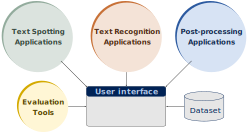
\includegraphics[width=0.6\textwidth]{figs/prototype-overview-simple.pdf}
    \caption{Overview of the main components of the prototype. The text spotting applications refer to methods used for detecting candidate regions in a scene, while the post-processing methods are used to refine detection results. The text recognition applications provide the components responsible for recognizing texts found within detected regions.}
    \label{fig:prototype-overview-simple}
\end{figure}

We organized the remainder of this document as follows: Section~\ref{sec:overview} provides an overview of the prototype; Section~\ref{sec:usage-scenario} presents a comprehensive usage scenario of the prototype, concerning the execution of different end-to-end recognition methods; finally, Section~\ref{sec:conclusions} presents our final remarks and directions for future investigations.